 \documentclass{article}

\usepackage{tikz} 
\usetikzlibrary{automata, positioning, arrows} 

\usepackage{amsthm}
\usepackage{amsfonts}
\usepackage{amsmath}
\usepackage{amssymb}
\usepackage{fullpage}
\usepackage{color}
\usepackage{parskip}
\usepackage{hyperref}
  \hypersetup{
    colorlinks = true,
    urlcolor = blue,
    linkcolor= blue,
    citecolor= blue,
    filecolor= blue,
    }
    
\usepackage{listings}
\usepackage[utf8]{inputenc}                                                    
\usepackage[T1]{fontenc}                                                       

\definecolor{dkgreen}{rgb}{0,0.6,0}
\definecolor{gray}{rgb}{0.5,0.5,0.5}
\definecolor{mauve}{rgb}{0.58,0,0.82}

\lstset{frame=tb,
  language=haskell,
  aboveskip=3mm,
  belowskip=3mm,
  showstringspaces=false,
  columns=flexible,
  basicstyle={\small\ttfamily},
  numbers=none,
  numberstyle=\tiny\color{gray},
  keywordstyle=\color{blue},
  commentstyle=\color{dkgreen},
  stringstyle=\color{mauve},
  breaklines=true,
  breakatwhitespace=true,
  tabsize=3
}

\newtheoremstyle{theorem}
  {\topsep}{\topsep}{\itshape\/}{0pt}{\bfseries}{.}{5pt plus 1pt minus 1pt}{}
\theoremstyle{theorem} 
   \newtheorem{theorem}{Theorem}[section]
   \newtheorem{corollary}[theorem]{Corollary}
   \newtheorem{lemma}[theorem]{Lemma}
   \newtheorem{proposition}[theorem]{Proposition}
\theoremstyle{definition}
   \newtheorem{definition}[theorem]{Definition}
   \newtheorem{example}[theorem]{Example}
\theoremstyle{remark}    
  \newtheorem{remark}[theorem]{Remark}

\setcounter{tocdepth}{3}
\setcounter{secnumdepth}{3}

\title{CPSC-354 Report}
\author{Jonathan Karam \\ Chapman University}

\date{\today} 

\begin{document}

\maketitle

\begin{abstract}
This report is a collection of notes, discussions, and homework solutions for CPSC 354. 
Homework 1 discusses the MIU puzzle and proves why \texttt{MI} cannot become \texttt{MU}. 
Homework 2 introduces abstract rewriting systems (ARS), includes TikZ diagrams, and classifies systems by termination, confluence, and unique normal forms. 
Homework 3 studies a rewriting system over $\{a,b\}$ and explores its equivalence classes and termination.
Homework 4 proves termination of two classic algorithms using measure functions.
Homework 5 evaluates a small $\lambda$-calculus ``workout'' using $\alpha$- and $\beta$-rules, with notes connecting these ideas to modern languages.
Homework 6 develops fixpoints and recursion: we compute \texttt{fact 3} step-by-step with the rules for \texttt{fix}, \texttt{let}, and \texttt{let rec}, and give a Y-combinator encoding of factorial.
Week 7 covers grammars, parse trees, and ASTs with full derivation trees.
Week 8 connects the Natural Number Game (Tutorial World) to natural-language proofs and Lean tactics, with scripts for Levels 5--8 and a short class-notes discussion.
Week 9 proves an Addition World lemma in two different styles (lemma-driven and inductive).
\textbf{Week 10 adds one-line solutions for the Lean Logic Game (Implication World) Levels 6--9.}
\textbf{Week 11 completes the Lean Logic \emph{Negation Tutorial} with one-line solutions for Levels 9--12, plus brief notes and a Discord question.}
\textbf{Week 12 analyzes the Towers of Hanoi puzzle, including the first move for $n=3$, a recursive algorithm that solves the puzzle for any $n$, and class questions about recursion vs iteration and stack depth.}
\textbf{Week 13 uses the Python-based $\lambda$-calculus interpreter: I design simple test cases, look at capture-avoiding substitution, find a minimal non-terminating example, and answer questions about evaluation strategies, divergence, and using the debugger.}
\end{abstract}

\tableofcontents

\section{Introduction}
This report documents my learning week by week. 
Each section includes my notes and discussions of the lecture topics, followed by my homework solutions.
The purpose is to show understanding, practice writing in \LaTeX{}, and explain the material in my own words.

\section{Week 1: The MIU Puzzle}

\subsection{Notes and Discussion}
The first week introduced the MIU puzzle, created by Douglas Hofstadter. 
It is a formal system that begins with the word \texttt{MI} and has four rules. 
The puzzle asks whether it is possible to reach \texttt{MU}. 
This is important because it shows how formal systems can be analyzed with invariants, a key concept in logic and computer science.

\subsection{Homework}
\textbf{Rules:}
\begin{enumerate}
  \item If a string ends with \texttt{I}, add a \texttt{U}.
  \item If a string starts with \texttt{M}, double the part after \texttt{M}.
  \item Replace \texttt{III} with \texttt{U}.
  \item Remove \texttt{UU}.
\end{enumerate}

\textbf{Why \texttt{MI} cannot become \texttt{MU}:}  
Let $\#I(w)$ be the number of \texttt{I}'s in $w$. Initially $\#I(\texttt{MI})=1$. 
Each rule preserves $\#I(w) \pmod{3}$:
\begin{itemize}
  \item Rule 1: no effect.
  \item Rule 2: doubles the count, $1 \mapsto 2$, never $0 \pmod 3$.
  \item Rule 3: subtracts 3, same remainder.
  \item Rule 4: no effect.
\end{itemize}
Thus $\#I(w) \pmod{3}$ is invariant. Since \texttt{MU} has $\#I=0$, it cannot be reached.

\textbf{Deeper explanation:}  
The invariant argument proves that all reachable words have I-count $\equiv 1$ or $2 \pmod{3}$, never 0.  
The first letter $M$ never disappears, so all reachable words start with $M$.  
Another way: define a homomorphism $h(M)=0, h(U)=0, h(I)=1 \pmod 3$. 
Every rule preserves $h$, so $h(\texttt{MI})=1$ and $h(\texttt{MU})=0$. Contradiction.  

\section{Week 2: Abstract Rewriting Systems}

\subsection{Notes and Discussion}
This week focused on abstract rewriting systems. 
An ARS consists of a set $A$ and a relation $R$. 
We ask whether rewriting always stops (termination), whether different rewrite paths can rejoin (confluence), and whether elements end up in unique normal forms.

\subsection{Homework}
\emph{Same problem statement as before:} draw each ARS and decide termination, confluence, and whether the system has \emph{unique normal forms for all elements} (UN-for-all).

\subsubsection*{Examples (drawings unchanged)}
\begin{tikzpicture}
  % Example 1
\end{tikzpicture}

\textbf{1: $A=\{\}, R=\{\}$} (empty system)

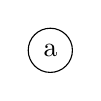
\begin{tikzpicture}
  \node[draw,circle] (a) at (0,0) {a};
\end{tikzpicture}

\textbf{2: $A=\{a\}, R=\{\}$}

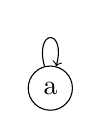
\begin{tikzpicture}
  \node[draw,circle] (a) at (0,0) {a};
  \draw[->] (a) to[loop above] (a);
\end{tikzpicture}

\textbf{3: $A=\{a\}, R=\{(a,a)\}$}

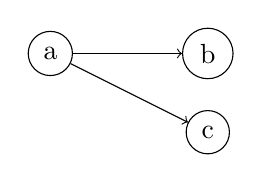
\begin{tikzpicture}
  \node[draw,circle] (a) at (0,0) {a};
  \node[draw,circle] (b) at (2,0) {b};
  \node[draw,circle] (c) at (2,-1) {c};
  \draw[->] (a) -- (b);
  \draw[->] (a) -- (c);
\end{tikzpicture}

\textbf{4: $A=\{a,b,c\}, R=\{(a,b),(a,c)\}$}

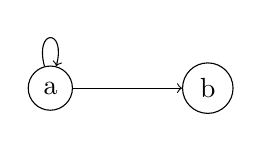
\begin{tikzpicture}
  \node[draw,circle] (a) at (0,0) {a};
  \node[draw,circle] (b) at (2,0) {b};
  \draw[->] (a) to[loop above] (a);
  \draw[->] (a) -- (b);
\end{tikzpicture}

\textbf{5: $A=\{a,b\}, R=\{(a,a),(a,b)\}$}

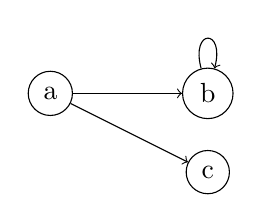
\begin{tikzpicture}
  \node[draw,circle] (a) at (0,0) {a};
  \node[draw,circle] (b) at (2,0) {b};
  \node[draw,circle] (c) at (2,-1) {c};
  \draw[->] (a) -- (b);
  \draw[->] (a) -- (c);
  \draw[->] (b) to[loop above] (b);
\end{tikzpicture}

\textbf{6: $A=\{a,b,c\}, R=\{(a,b),(b,b),(a,c)\}$}

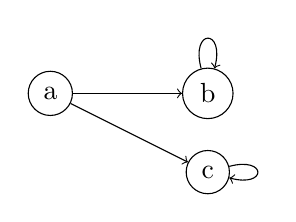
\begin{tikzpicture}
  \node[draw,circle] (a) at (0,0) {a};
  \node[draw,circle] (b) at (2,0) {b};
  \node[draw,circle] (c) at (2,-1) {c};
  \draw[->] (a) -- (b);
  \draw[->] (a) -- (c);
  \draw[->] (b) to[loop above] (b);
  \draw[->] (c) to[loop right] (c);
\end{tikzpicture}

\textbf{7: $A=\{a,b,c\}, R=\{(a,b),(b,b),(a,c),(c,c)\}$}

\subsubsection*{Classification (solutions rewritten)}
We now use \textbf{UN-for-all}: every element must have a (unique) normal form.

\[
\begin{array}{c|c|c|c|l}
\text{ARS} & \text{Terminating} & \text{Confluent} & \text{UN-for-all} & \text{Why} \\\hline
1 & \text{Yes} & \text{Yes} & \text{Yes} & \text{Nothing rewrites (vacuous).} \\
2 & \text{Yes} & \text{Yes} & \text{Yes} & a \text{ is already normal and unique.} \\
3 & \text{No} & \text{Yes} & \text{No}  & a \to a \text{ forever; } a \text{ has no NF.} \\
4 & \text{Yes} & \text{No}  & \text{No}  & a\to b,\,a\to c \text{ (two distinct NFs).} \\
5 & \text{No} & \text{Yes} & \text{Yes} & a\to b,\; b \text{ normal; both end at } b. \\
6 & \text{No} & \text{No}  & \text{No}  & b \text{ loops; } a\to c \text{ NF, not joinable with } b. \\
7 & \text{No} & \text{No}  & \text{No}  & b,c \text{ loop; no element has an NF.} \\
\end{array}
\]

\paragraph{Remarks.}
\begin{itemize}
  \item Non-termination alone does not rule out UN-for-all (see 5), but any element without an NF breaks it (3,6,7).
  \item In terminating ARSs, confluence $\Rightarrow$ UN-for-all (every element reaches a unique NF).
  \item Item 4 is the canonical ``diamond failure'': two different normal forms reachable from the same source.
\end{itemize}

\section{Week 3: Strings over \{a,b\}}

\subsection{Notes and Discussion}
We studied rewriting rules over alphabet $\{a,b\}$. 
This shows how simple systems can classify strings into equivalence classes. 
We also saw how orienting rules one way can make a system terminating without changing equivalence.

\subsection{Homework 3}
\textbf{Exercise 5 rules:}
\[
ab \to ba,\quad ba \to ab,\quad aa \to \varepsilon,\quad b \to \varepsilon
\]

Examples: \texttt{abba} $\to$ \texttt{aa} $\to$ $\varepsilon$.  
\texttt{bababa} $\to$ \texttt{aaa} $\to$ \texttt{a}.  

Not terminating because swaps loop.  
Equivalence classes: even number of $a$’s $\to \varepsilon$, odd $\to a$.  
Normal forms: $\varepsilon, a$.  
Fix: orient $ba \to ab$ only.  

\textbf{Exercise 5b rules:}
\[
ab \leftrightarrow ba,\quad aa \to a,\quad b \to \varepsilon
\]

Examples: \texttt{abba} $\to$ \texttt{a}. \texttt{bababa} $\to$ \texttt{a}.  

Equivalence: all $b$ vanish, runs of $a$ collapse to one $a$.  
Classes: $\{\varepsilon,a\}$.  
Fix: orient swaps, keep $aa \to a$ and $b \to \varepsilon$.  

\section{Week 4: Measure Functions and Termination}

\subsection{Notes and Discussion}
This week we looked at \emph{measure functions} to prove that algorithms terminate.
A measure maps the state of a computation to a value in a well-founded set (usually the natural numbers) and must
\emph{strictly decrease} with every loop iteration or recursive call. Because there are no infinite descending chains in a well-founded set, the computation must eventually stop.

\textbf{Scope note:} Here we define a measure and show it strictly decreases.

\paragraph{Class notes invariant proof that Euclid returns $\gcd$.}
\begin{itemize}
  \item \textbf{Key fact.} $\gcd(a,b)=\gcd\!\big(b,\,a-qb\big)$ for any integer $q$.
  \item \textbf{Update.} Writing $a=qb+r$ with $r=a\bmod b$, the step $(a,b)\mapsto(b,r)$ keeps the gcd unchanged.
  \item \textbf{Invariant.} Before each loop test: $\gcd(a,b)=\gcd(a_0,b_0)$.
  \item \textbf{End.} When $b=0$, $\gcd(a_0,b_0)=\gcd(a,0)=|a|$, the returned value.
\end{itemize}

\subsection{Homework 4}

\subsubsection*{HW 4.1}
\textbf{Problem.} Considering
\begin{lstlisting}[language=Python]
while b != 0:
    temp = b
    b = a % b
    a = temp
return a
\end{lstlisting}
Under which conditions does this algorithm always terminate? Find a measure function and prove termination.

\medskip
\textbf{Answer.}  
This is the classical Euclidean algorithm for $\gcd(a,b)$. It always terminates provided that
\[
a,b \in \mathbb{Z}\quad\text{and}\quad b \ge 0,
\]
and we interpret \texttt{\%} as the mathematical remainder with $0 \le a \bmod b < b$ for $b>0$. If the inputs are negative, replace them once by $|a|,|b|$; this preserves $\gcd$ and satisfies the condition.

\paragraph{Measure function.}
Let the program state be the pair $(a,b)$ with $b \ge 0$. Define
\[
\mu(a,b) \;=\; b \in \mathbb{N}.
\]

\paragraph{Strict decrease.}
In an iteration with $b>0$ we set $b' = a \bmod b$. By definition of remainder,
\[
0 \le b' < b.
\]
Therefore $\mu(a',b') = b' < b = \mu(a,b)$. Hence $\mu$ strictly decreases on every loop step.

\paragraph{Well-foundedness and termination.}
$\mu$ maps states to the natural numbers with the usual $<$, which is well founded.  
Because $\mu$ strictly decreases whenever the loop body executes, the loop can execute only finitely many times; eventually $b=0$ and the algorithm returns. \qed

\begin{remark}
The algorithm not only terminates; it returns $\gcd(a,b)$. This follows from the class note invariant above and $\gcd(a,0)=|a|$.
\end{remark}

\subsubsection*{HW 4.2}
\textbf{Problem.} Consider the fragment of merge sort:
\begin{lstlisting}[language=Python]
def merge_sort(arr, left, right):
    if left >= right:
        return
    mid = (left + right) // 2
    merge_sort(arr, left, mid)
    merge_sort(arr, mid + 1, right)
    merge(arr, left, mid, right)
\end{lstlisting}
Prove that
\[
\varphi(left,right) \;=\; right - left + 1
\]
is a measure function for \texttt{merge\_sort}.

\medskip
\textbf{Answer.}
We show that every recursive call is made with a \emph{strictly smaller} measure and that the measure is bounded below by $0$.

\paragraph{Well-founded codomain.}
$\varphi(left,right)$ is a nonnegative integer whenever $left\le right$, so the codomain is $\mathbb{N}$ with the usual $<$ (well-founded).

\paragraph{Base case.}
If $left \ge right$, the function returns immediately. In this case $\varphi \le 1$, and there are no recursive calls.

\paragraph{Decrease for recursive calls.}
Assume $left < right$ and let $n = \varphi(left,right) = right-left+1 \ge 2$. With
\[
mid = \left\lfloor \frac{left+right}{2} \right\rfloor,
\]
the first recursive call is on $[left,\,mid]$ and the second on $[mid+1,\,right]$. Their measures are
\[
\varphi(left,mid) = mid - left + 1, \qquad
\varphi(mid+1,right) = right - mid.
\]
Because $left \le mid < right$, we have
\[
1 \le \varphi(left,mid) \le \left\lceil \frac{n}{2}\right\rceil < n,\qquad
1 \le \varphi(mid+1,right) \le \left\lfloor \frac{n}{2}\right\rfloor < n.
\]
Thus each recursive call receives strictly smaller measure than $n$.

\paragraph{Conclusion.}
Every chain of recursive calls strictly decreases $\varphi$ and cannot be infinite in $\mathbb{N}$. Therefore \texttt{merge\_sort} terminates. \qed

\section{Week 5: Lambda Calculus Foundations}

\subsection{Notes and Discussion}
\begin{itemize}
  \item \textbf{Self-application and computation.} Terms like $(\lambda x.\,xx)(\lambda x.\,xx)$ show that functions can take \emph{code as data}. This enables iteration/recursion encodings (fixed points) and explains why untyped $\lambda$ can express non-termination.
  \item \textbf{Where $\lambda$ shines.} Useful for building \emph{minimal cores}: interpreters, proof assistants, type checkers, compiler IRs, and reasoning about higher-order functions. It models substitution, scope, closures, and evaluation precisely.
  \item \textbf{Composition and numerals.} Church numerals encode iteration: $\mathbf{n}\,f\,x = f^{n}x$. Function composition $(f \circ g)$ corresponds to multiplying numerals: $(\mathbf{m}\circ\mathbf{n})\,f\,x = f^{mn}x$. Plain application behaves like \emph{exponentiation in reverse order}: $\mathbf{m}\,\mathbf{n} = \mathbf{n}^{\,\mathbf{m}}$ (apply $\mathbf{m}$ times), so $\mathbf{2}\,\mathbf{3}=\mathbf{9}$ and $\mathbf{3}\,\mathbf{2}=\mathbf{8}$.
  \item \textbf{Confluence (Church–Rosser).} If a term reduces to two results, there exists a common reduct. Meaning: evaluation order doesn’t affect the final normal form (when it exists). Languages borrow this idea to justify equational reasoning and optimizations.
  \item \textbf{From $\lambda$ to languages.} Add types (safety), effects (state, I/O), data types, and evaluation strategy to get modern languages. Typed $\lambda$-cal\-culi (System~F, Hindley–Milner) underlie ML/Haskell; effect systems/monads model side effects.
  \item \textbf{Haskell links.} Purity, first-class functions, laziness (normal-order–like), algebraic data types, and type inference all line up with typed $\lambda$-calculus. Monads/Applicatives are structured ways to compose computations.
  \item \textbf{Names and $\alpha$-conversion.} Variables need not be single letters; names are irrelevant up to $\alpha$-equivalence (consistent renaming). Modern languages reflect this via lexical scope, hygienic macros, and compiler renaming to avoid capture.
  \item \textbf{The role of $\alpha$ in practice.} Compilers implement renaming and fresh-name generation to maintain scope hygiene (e.g., SSA form, macro expansion).
  \item \textbf{Termination and type systems.} Untyped $\lambda$ allows non-termination (Y-combinator). Total languages (Coq/Agda) \emph{forbid} general recursion by checking termination via structural/lexicographic and multivariate measures; complex patterns (exponential, multi-dimension decrease) are handled with well-founded orders and sized types.
  \item \textbf{Original intent.} Church invented $\lambda$ for the foundations of mathematics and to study effective computability—leading to Church–Turing thesis.
  \item \textbf{Recursion vs loops.} Prefer recursion for recursive structure or immutability; prefer loops for in-place iteration or where tail recursion isn’t optimized.
\end{itemize}

\subsection{Homework 5: Lambda Calculus Workout}

\subsubsection*{Problem}
Evaluate (practice $\alpha$ and $\beta$ rules; match parentheses):
\[
\Big(\lambda f.\,\lambda x.\,f(f\,x)\Big)\;
\Big(\lambda f.\,\lambda x.\,f(f(f\,x))\Big).
\]

\subsubsection*{Solution}
Let
\[
\mathbf{two} \equiv \lambda f.\lambda x.\,f(fx),\qquad
\mathbf{three} \equiv \lambda f.\lambda x.\,f(f(fx)).
\]
Then
\[
\mathbf{two}\;\mathbf{three}
\;\xrightarrow{\beta}\;
\lambda x.\,\mathbf{three}\,(\mathbf{three}\,x).
\]
Compute:
\[
\mathbf{three}\,x \xrightarrow{\beta} \lambda y.\,x(x(x\,y)),
\qquad
\mathbf{three}\,(\lambda y.\,x(x(x\,y))) \xrightarrow{\beta} \lambda z.\,x^{9}z.
\]
Therefore
\[
\boxed{\lambda x.\lambda z.\,x^{9}z}
\]
which is the Church numeral $\mathbf{nine}$.
(And $\mathbf{3}\,\mathbf{2}=\mathbf{8}$ because $\mathbf{m}\,\mathbf{n}=\mathbf{n}^{\,\mathbf{m}}$.)

% ============================
\section{Week 6: Fixpoints and Recursion}
% ============================

\subsection{Class Notes \& Discussion}
This section responds concisely to discussion questions from class.

\begin{enumerate}
  \item \textbf{Reducing inside larger expressions and step rules for \texttt{fix}, \texttt{let}, \texttt{if}.}
  We use \emph{evaluation contexts}: reduce inside the syntactic position allowed by the strategy (e.g., call-by-value reduces the scrutinee of \texttt{if}, the bound expression of \texttt{let}, and the argument to \texttt{fix} until it is a $\lambda$). Rules:
  \[
  \mathrm{fix}\ F \;\to\; F(\mathrm{fix}\ F),\qquad
  \mathrm{let}\ x=e_1\ \mathrm{in}\ e_2 \;\to\; (\lambda x.\,e_2)\,e_1,\qquad
  \mathrm{if}\ \text{true}\ \text{then}\ e_1\ \text{else}\ e_2 \to e_1.
  \]
  Contexts justify each inner step when \texttt{fix}, \texttt{let}, or \texttt{if} appears inside a bigger term.

  \item \textbf{Fixpoint combinator and recursion.}
  A combinator $Y$ with $YF = F(YF)$ provides a value $YF$ that is a fixed point of $F$. If $F$ encodes one step of a recursive definition, $YF$ is its recursive solution. Languages often bake this in as a primitive \texttt{fix}.

  \item \textbf{Factorial with $Y$ instead of \texttt{fix}.}
  \[
  \mathrm{fact} \;\equiv\; Y\,(\lambda f.\,\lambda n.\ \mathrm{if}\ n=0\ \mathrm{then}\ 1\ \mathrm{else}\ n \cdot f(n-1)).
  \]

  \item \textbf{Typed vs untyped.} In typed, strongly normalizing calculi, general $Y$ breaks termination; practical languages use explicit recursion with typing restrictions, or domain-theoretic semantics for effects.
\end{enumerate}

\subsection{Homework 6}

We use these computation rules:
\[
\mathrm{fix}\ F \to F(\mathrm{fix}\ F),\quad
\mathrm{let}\ x=e_1\ \mathrm{in}\ e_2 \to (\lambda x.\,e_2)\,e_1,\quad
\mathrm{let\ rec}\ f=e_1\ \mathrm{in}\ e_2 \to \mathrm{let}\ f=(\mathrm{fix}\ (\lambda f.\,e_1))\ \mathrm{in}\ e_2.
\]

\subsubsection*{Problem A: Compute \texttt{fact 3}}
Start with
\[
\mathrm{let\ rec}\ \mathrm{fact} = \lambda n.\ \mathrm{if}\ n=0\ \mathrm{then}\ 1\ \mathrm{else}\ n * \mathrm{fact}(n-1)\ \mathrm{in}\ \mathrm{fact}\ 3.
\]

\noindent\textbf{Derivation}
\[
\begin{aligned}
&\mathrm{let\ rec}\ \mathrm{fact}=\lambda n.\ \mathrm{if}\ n=0\ \mathrm{then}\ 1\ \mathrm{else}\ n * \mathrm{fact}(n-1)\ \mathrm{in}\ \mathrm{fact}\ 3\\
\to\ &\text{\textbf{(def of let rec)}}\\
&\mathrm{let}\ \mathrm{fact}=\mathrm{fix}\ (\lambda f.\ \lambda n.\ \mathrm{if}\ n=0\ \mathrm{then}\ 1\ \mathrm{else}\ n * f(n-1))\ \mathrm{in}\ \mathrm{fact}\ 3\\
\to\ &\text{\textbf{(def of let)}}\\
&(\lambda \mathrm{fact}.\ \mathrm{fact}\ 3)\ \big(\mathrm{fix}\ F\big)
\quad\text{where }F \equiv \lambda f.\ \lambda n.\ \mathrm{if}\ n=0\ \mathrm{then}\ 1\ \mathrm{else}\ n * f(n-1)\\
\to\ &\text{\textbf{($\beta$; substitute $\mathrm{fix}\ F$ for fact)}}\\
&(\mathrm{fix}\ F)\ 3\\
\to\ &\text{\textbf{(def of fix)}}\\
&\big(F(\mathrm{fix}\ F)\big)\ 3\\
\to\ &\text{\textbf{($\beta$)}}\\
&(\lambda n.\ \mathrm{if}\ n=0\ \mathrm{then}\ 1\ \mathrm{else}\ n * (\mathrm{fix}\ F)(n-1))\ 3\\
\to\ &\text{\textbf{($\beta$; substitute $3$ for $n$)}}\\
&\mathrm{if}\ 3=0\ \mathrm{then}\ 1\ \mathrm{else}\ 3 * (\mathrm{fix}\ F)(2)\\
\to\ &\text{\textbf{(def of if)}}\\
&3 * (\mathrm{fix}\ F)(2)\\
\to\ &\text{\textbf{(def of fix)}}\\
&3 * \big(F(\mathrm{fix}\ F)\big)\,2\\
\to\ &\text{\textbf{($\beta$)}}\\
&3 * (\lambda n.\ \mathrm{if}\ n=0\ \mathrm{then}\ 1\ \mathrm{else}\ n * (\mathrm{fix}\ F)(n-1))\ 2\\
\to\ &\text{\textbf{($\beta$; substitute $2$ for $n$)}}\\
&3 * \big(\mathrm{if}\ 2=0\ \mathrm{then}\ 1\ \mathrm{else}\ 2 * (\mathrm{fix}\ F)(1)\big)\\
\to\ &\text{\textbf{(def of if)}}\\
&3 * \big(2 * (\mathrm{fix}\ F)(1)\big)\\
\to\ &\text{\textbf{(def of fix)}}\\
&3 * \big(2 * \big(F(\mathrm{fix}\ F)\big)\,1\big)\\
\to\ &\text{\textbf{($\beta$)}}\\
&3 * \big(2 * (\lambda n.\ \mathrm{if}\ n=0\ \mathrm{then}\ 1\ \mathrm{else}\ n * (\mathrm{fix}\ F)(n-1))\ 1\big)\\
\to\ &\text{\textbf{($\beta$; substitute $1$ for $n$)}}\\
&3 * \big(2 * \big(\mathrm{if}\ 1=0\ \mathrm{then}\ 1\ \mathrm{else}\ 1 * (\mathrm{fix}\ F)(0)\big)\big)\\
\to\ &\text{\textbf{(def of if)}}\\
&3 * \big(2 * \big(1 * (\mathrm{fix}\ F)(0)\big)\big)\\
\to\ &\text{\textbf{(def of fix)}}\\
&3 * \big(2 * \big(1 * \big(F(\mathrm{fix}\ F)\big)\,0\big)\big)\\
\to\ &\text{\textbf{($\beta$)}}\\
&3 * \big(2 * \big(1 * (\lambda n.\ \mathrm{if}\ n=0\ \mathrm{then}\ 1\ \mathrm{else}\ n * (\mathrm{fix}\ F)(n-1))\ 0\big)\big)\\
\to\ &\text{\textbf{($\beta$; substitute $0$ for $n$)}}\\
&3 * \big(2 * \big(1 * (\mathrm{if}\ 0=0\ \mathrm{then}\ 1\ \mathrm{else}\ 0 * (\mathrm{fix}\ F)(-1))\big)\big)\\
\to\ &\text{\textbf{(def of if)}}\\
&3 * \big(2 * (1 * 1)\big) \;=\; 3 * 2 * 1 \;=\; \boxed{6}.
\end{aligned}
\]

\subsubsection*{Problem B: Y-combinator factorial and one unfold}
Let
\[
Y \equiv \lambda g.\ (\lambda x.\ g(x\,x))(\lambda x.\ g(x\,x)),\quad
G \equiv \lambda f.\ \lambda n.\ \mathrm{if}\ n=0\ \mathrm{then}\ 1\ \mathrm{else}\ n * f(n-1).
\]
Define $\mathrm{fact} \equiv YG$. Then
\[
\mathrm{fact} \;=\; YG \;\to\; G(YG) \;=\; \lambda n.\ \mathrm{if}\ n=0\ \mathrm{then}\ 1\ \mathrm{else}\ n * (YG)(n-1),
\]
which is exactly one recursive ``unfold''.

\begin{remark}
In total/strongly normalizing typed calculi, $Y$ cannot be defined without sacrificing termination. Practical languages provide explicit recursion or \texttt{fix}, often with typing restrictions.
\end{remark}

% ============================
\section{Week 7: Grammars, Parse Trees, and ASTs}
% ============================

\subsection{Class Notes \& Discussion}

\begin{itemize}
  \item \textbf{Fixed-point combinators and performance.} Using $Y$/\texttt{fix} introduces an extra unfolding step ($YF \to F(YF)$). Named recursion or \texttt{let rec} generally performs better since the compiler can optimize it directly without creating closures on each call.
  \item \textbf{LLMs as metaprograms.} Large language models can be viewed as metaprograms that translate semantics (intent or meaning) into code. However, they do not replace the traditional compiler pipeline—semantic interpretation, parsing, optimization, and execution still occur afterward.
  \item \textbf{Lisp and syntax readability.} Lisp’s simple S-expression syntax gives programmers direct access to abstract syntax, making metaprogramming and macro systems easier to implement. The trade-off is reduced human readability but increased ease of parsing for machines.
  \item \textbf{Ambiguous grammars.} Ambiguity in grammars can make parsing inconsistent; precedence and associativity rules often disambiguate.
  \item \textbf{Parse trees vs.\ ASTs.} Parse trees include every token; ASTs compress away redundant structure (e.g., parentheses) to expose semantics for analysis and code generation.
\end{itemize}

\subsection{Homework 7: Context-Free Grammar and Derivation Trees}

Grammar:
\[
\begin{array}{rcl}
\text{Exp} &\to& \text{Exp}\;+\;\text{Exp1}\ \mid\ \text{Exp1}\\
\text{Exp1} &\to& \text{Exp1}\;*\;\text{Exp2}\ \mid\ \text{Exp2}\\
\text{Exp2} &\to& \text{Integer}\ \mid\ (\,\text{Exp}\,)
\end{array}
\]

\paragraph{(a) \texttt{2+1}}
\begin{center}
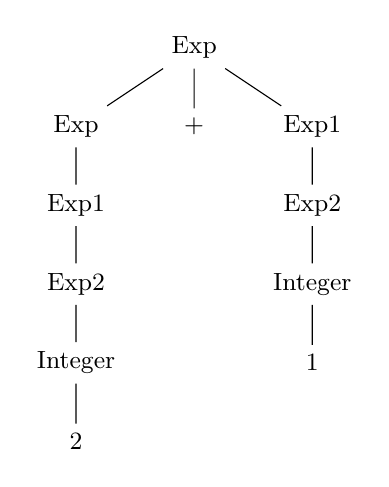
\begin{tikzpicture}[grow=down,level distance=10mm, every node/.style={font=\small}]
\node{Exp}
 child{ node{Exp}
   child{ node{Exp1}
     child{ node{Exp2}
       child{ node{Integer} child{ node{$2$} } }}}}
 child{ node{$+$} }
 child{ node{Exp1}
   child{ node{Exp2}
     child{ node{Integer} child{ node{$1$} } }}};
\end{tikzpicture}
\end{center}

\paragraph{(b) \texttt{1+2*3}}
\begin{center}
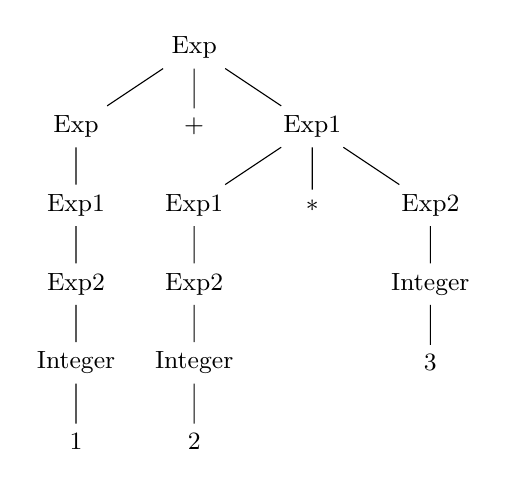
\begin{tikzpicture}[grow=down,level distance=10mm, every node/.style={font=\small}]
\node{Exp}
 child{ node{Exp}
   child{ node{Exp1}
     child{ node{Exp2}
       child{ node{Integer} child{ node{$1$} } }}}}
 child{ node{$+$} }
 child{ node{Exp1}
   child{ node{Exp1}
     child{ node{Exp2}
       child{ node{Integer} child{ node{$2$} } }}}
   child{ node{$*$} }
   child{ node{Exp2}
     child{ node{Integer} child{ node{$3$} } }}};
\end{tikzpicture}
\end{center}

\paragraph{(c) \texttt{1+(2*3)}}
\begin{center}
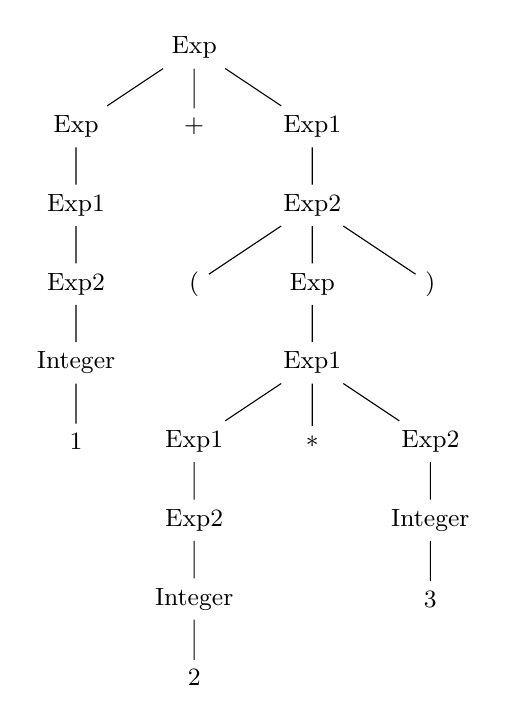
\begin{tikzpicture}[grow=down,level distance=10mm, every node/.style={font=\small}]
\node{Exp}
 child{ node{Exp}
   child{ node{Exp1}
     child{ node{Exp2}
       child{ node{Integer} child{ node{$1$} } }}}}
 child{ node{$+$} }
 child{ node{Exp1}
   child{ node{Exp2}
     child{ node{$($} }
     child{ node{Exp}
       child{ node{Exp1}
         child{ node{Exp1}
           child{ node{Exp2}
             child{ node{Integer} child{ node{$2$} } }}}
         child{ node{$*$} }
         child{ node{Exp2}
           child{ node{Integer} child{ node{$3$} } }}}}
     child{ node{$)$} }}};
\end{tikzpicture}
\end{center}

\paragraph{(d) \texttt{(1+2)*3}}
\begin{center}
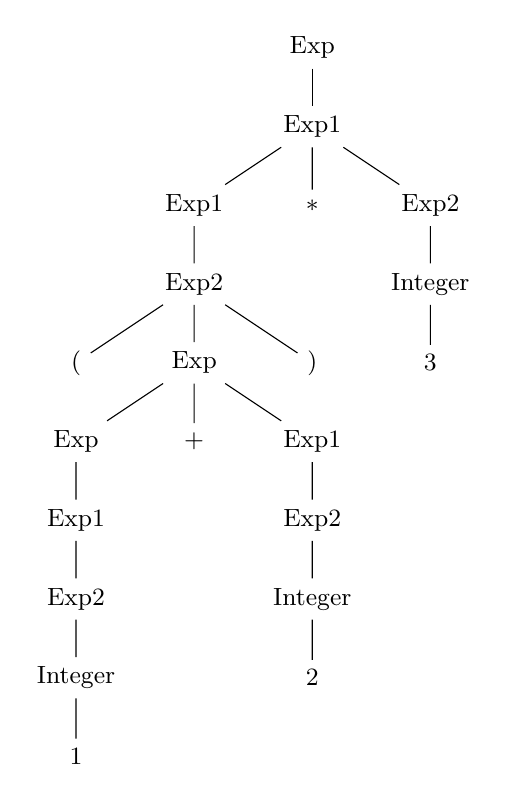
\begin{tikzpicture}[grow=down,level distance=10mm, every node/.style={font=\small}]
\node{Exp}
 child{ node{Exp1}
   child{ node{Exp1}
     child{ node{Exp2}
       child{ node{$($} }
       child{ node{Exp}
         child{ node{Exp}
           child{ node{Exp1}
             child{ node{Exp2}
               child{ node{Integer} child{ node{$1$} } }}}}
         child{ node{$+$} }
         child{ node{Exp1}
           child{ node{Exp2}
             child{ node{Integer} child{ node{$2$} } }}}}
       child{ node{$)$} }}}
   child{ node{$*$} }
   child{ node{Exp2}
     child{ node{Integer} child{ node{$3$} } }}};
\end{tikzpicture}
\end{center}

\paragraph{(e) \texttt{1+2*3+4*5+6}}
\begin{center}
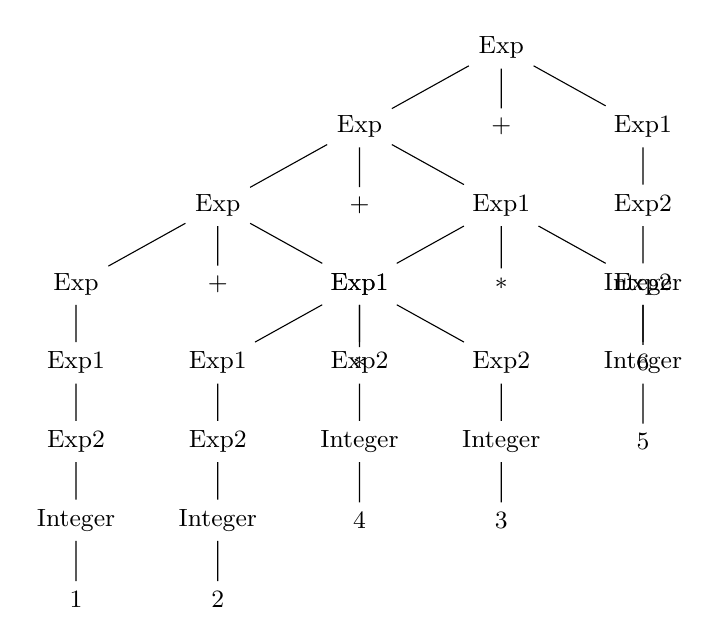
\begin{tikzpicture}[grow=down,level distance=10mm, sibling distance=18mm, every node/.style={font=\small}]
\node{Exp}
  child{ node{Exp}
    child{ node{Exp}
      child{ node{Exp}
        child{ node{Exp1}
          child{ node{Exp2}
            child{ node{Integer} child{ node{$1$} } }}}}
      child{ node{$+$} }
      child{ node{Exp1}
        child{ node{Exp1}
          child{ node{Exp2}
            child{ node{Integer} child{ node{$2$} } }}}
        child{ node{$*$} }
        child{ node{Exp2}
          child{ node{Integer} child{ node{$3$} } }}}}
    child{ node{$+$} }
    child{ node{Exp1}
      child{ node{Exp1}
        child{ node{Exp2}
          child{ node{Integer} child{ node{$4$} } }}
        }
      child{ node{$*$} }
      child{ node{Exp2}
        child{ node{Integer} child{ node{$5$} } }}}}
  child{ node{$+$} }
  child{ node{Exp1}
    child{ node{Exp2}
      child{ node{Integer} child{ node{$6$} } }}};
\end{tikzpicture}
\end{center}

% ============================
\section{Week 8: Natural Number Game (Tutorial World)}
% ============================

\subsection{Notes \& Setup}
This task connects informal English proofs with formal Lean steps. In the Tutorial World we use facts like
\[
a+0=a,\qquad a+\mathrm{succ}(b)=\mathrm{succ}(a+b),\qquad 1=\mathrm{succ}(0),
\]
and finish goals by reflexivity (\texttt{rfl}) after rewriting.

\subsection{Selected Level Solutions (5--8)}
Below are minimal tactic scripts matching the in-game steps. (They are illustrative—other equivalent scripts also pass.)

\paragraph{Level 5 — Adding zero (right).}
\begin{lstlisting}[language=Haskell]
rw [add_zero b]
rw [add_zero c]
rfl
\end{lstlisting}

\paragraph{Level 6 — Careful rewriting.}
\begin{lstlisting}[language=Haskell]
rw [add_zero b]
rw [add_zero c]
rfl
\end{lstlisting}

\paragraph{Level 7 — Show  a + 1 = succ a.}
\begin{lstlisting}[language=Haskell]
rw [one_eq_succ_zero]
rw [add_succ]
rw [add_zero]
rfl
\end{lstlisting}

\paragraph{Level 8 — Compute 2 + 2 = 4.}
\begin{lstlisting}[language=Haskell]
-- Use 2 = succ 1 and 1 = succ 0, then unfold addition by add_succ
nth_rewrite 2 [two_eq_succ_one]
rw [add_succ 2]
nth_rewrite 1 [one_eq_succ_zero]
-- continue rewrites until the goal closes by rfl
\end{lstlisting}

\subsection{Class Notes \& Discussion}
\begin{itemize}
  \item \textbf{English vs.\ Lean proofs.} The Lean script mirrors an English proof by repeatedly replacing equals by equals (rewrite) until both sides are syntactically identical (\texttt{rfl}).
  \item \textbf{Core facts used.} Right identity of addition ($a+0=a$), right recursion ($a+\mathrm{succ}(b)=\mathrm{succ}(a+b)$), and numeral definitions ($1=\mathrm{succ}(0)$, $2=\mathrm{succ}(1)$).
  \item \textbf{Tactics as rules of inference.} Each \texttt{rw} corresponds to applying an equality as a substitution rule; the order of rewrites matters to expose the shape needed for the next lemma.
  \item \textbf{Why recursion on the right?} Defining $+$ by recursion on the second argument gives the simple law above and simplifies induction proofs on the right operand. Recursing on the left would require different lemmas (e.g., $\mathrm{succ}(a)+b=\mathrm{succ}(a+b)$) and different induction patterns.
  \item \textbf{Equality reasoning pattern.} Normalize numerals $\to$ unfold by recursive law \texttt{add\_succ} repeatedly $\to$ discharge with identities like \texttt{add\_zero} $\to$ finish with \texttt{rfl}.
\end{itemize}

% ============================
\section{Week 9: Addition World — Two Proofs \& Notes}
% ============================

\subsection{Notes \& Discussion (Q\&A)}

\paragraph{Boundary between definitional and propositional equality.}
\emph{Definitional} (or judgmental) equality is what the kernel reduces by computation/expansion and treats as the \emph{same term} (e.g.\ $\mathrm{Nat.add}\ a\ 0 \equiv a$, $\beta$-, $\delta$-, $\iota$-reductions). No proof object is needed; goals discharge by \texttt{rfl} or \texttt{simp} that performs computation.  
\emph{Propositional} equality (\texttt{Eq}) is a type inhabited by a proof term (e.g.\ a chain of rewrites) showing two \emph{a priori} different terms are equal; it is manipulated with lemmas like \texttt{add\_assoc}, \texttt{congrArg}, \texttt{calc}, etc. Intuition: definitional = computation; propositional = reasoning about equality beyond raw computation.

\paragraph{How $\mathbb{N}$’s inductive definition enables recursive $+$.}
With \texttt{inductive Nat | zero | succ : Nat → Nat}, primitive recursion defines $a + n$ by
\[
a + 0 \;=\; a,\qquad a + \mathrm{succ}(n) \;=\; \mathrm{succ}(a+n).
\]
Because \texttt{Nat.rec} (or \texttt{Nat.recOn}) eliminates on the second argument, the recursion equations above are \emph{defining} equalities that Lean can compute with directly.

\paragraph{SOLID in Lean / math-centric code.}
\begin{itemize}
  \item \textbf{S}ingle Responsibility: lemmas should prove exactly one fact; larger theorems compose small lemmas.
  \item \textbf{O}pen/Closed: extend the library with new lemmas (open), don’t rewrite core definitions (closed).
  \item \textbf{L}iskov Substitution: use typeclasses/instances (\texttt{Semiring}, \texttt{Monoid}) so theorems work for any instance.
  \item \textbf{I}nterface Segregation: expose minimal lemma interfaces; avoid giant \texttt{simp} sets that do too much.
  \item \textbf{D}ependency Inversion: reason at the level of algebraic interfaces rather than concrete \texttt{Nat} when possible.
\end{itemize}
Math-first programming prizes \emph{specification and proof}; SOLID maps well to clean lemma factoring and reusable abstractions.

\paragraph{Do all computational equality proofs end with \texttt{rfl}?}
No. Goals that are definitionally equal can close by \texttt{rfl}. Many “computational” goals can also finish via \texttt{simp} (using definitional rules like \texttt{Nat.add\_zero}, \texttt{Nat.add\_succ}). When non-computational rearrangements are needed (associativity/commutativity), we end with a lemma-driven chain or \texttt{simp}+\texttt{ring}-style tactics, not necessarily \texttt{rfl}.

\paragraph{Double induction for \texttt{add\_right\_comm} without \texttt{add\_comm}/\texttt{add\_assoc}?}
Yes in principle: prove $P(b,c): a+b+c=a+c+b$ for all $a$ by outer induction on $c$ and inner induction on $b$, using only the defining equations of $+$ and \texttt{succ} injectivity. It is longer and more technical in Lean because you must re-establish associativity-like rearrangements manually. Using standard lemmas is far shorter and idiomatic.

\paragraph{How logic/maths proofs deepen Lean and industry skills.}
They enforce precise specs, decomposition into lemmas (modularity), and automated checking (CI-like guarantees). This is directly transferable to testing, refactoring, and API design.

\paragraph{Induction vs.\ algebraic lemmas (comm/assoc).}
Being able to reach the same theorem both ways shows \emph{strategy choice}: induction exposes structure and well-founded decrease; lemma-based algebra leverages previously proved facts. In algorithm design this mirrors \emph{design space exploration}: choose recursion/iteration (structural approach) or algebraic transformations/identities (law-driven approach) depending on clarity and cost.

\medskip

\noindent\textit{Reference you cited (Tutorial World L8):} \url{https://adam.math.hhu.de/#/g/leanprover-community/nng4/world/Tutorial/level/8}

% -------------------------------------------------
\subsection{Homework 9: Addition World — Level 5 (two solutions)}
% -------------------------------------------------

\paragraph{Statement (as in Addition World, right-commuting the tail).}
We show, for all $a,b,c\in\mathbb{N}$,
\[
a + b + c \;=\; a + c + b\qquad\text{(often called \texttt{add\_right\_comm}).}
\]

\subsubsection*{Solution 1 (non-inductive, via lemmas).}
\begin{lstlisting}
-- Lean 4
theorem add_right_comm' (a b c : Nat) :
  a + b + c = a + c + b := by
  -- reshape: (a + b) + c  ≡  a + (b + c)
  calc
    a + b + c = a + (b + c) := by simp [Nat.add_assoc]
    _          = a + (c + b) := by simpa [Nat.add_comm]
    _          = a + c + b   := by simp [Nat.add_assoc]
\end{lstlisting}

\noindent\textbf{Pen-and-paper proof.}
Using associativity and commutativity of $+$,
\[
(a+b)+c \;=\; a+(b+c) \;=\; a+(c+b) \;=\; (a+c)+b.
\]
Each step is a standard ring law; hence $a+b+c = a+c+b$.

\subsubsection*{Solution 2 (inductive).}
We prove $P(c):\ \forall a b.\ a+b+c=a+c+b$ by induction on $c$.

\begin{lstlisting}
-- Lean 4
theorem add_right_comm_ind (a b c : Nat) :
  a + b + c = a + c + b := by
  induction c with
  | zero =>
      -- a + b + 0 = a + 0 + b
      simp [Nat.add_assoc, Nat.add_zero, Nat.zero_add]
  | succ c ih =>
      -- goal: a + b + succ c = a + succ c + b
      -- use the recursion equation for addition on the right argument
      -- x + succ c = succ (x + c)
      simp [Nat.add_assoc, ih]
\end{lstlisting}

\noindent\textbf{Pen-and-paper proof (matching the code).}
Define $P(c)\!:\!\forall a,b,\ (a+b)+c=(a+c)+b$.  
\emph{Base $c=0$:} $(a+b)+0=a+b=a+0+b$ by $x+0=x$ and $0+x=x$.  
\emph{Step $c\mapsto c+1$:}
\[
\begin{aligned}
(a+b)+(c+1) &= \mathrm{succ}\big((a+b)+c\big) &&\text{(def.\ of $+$)}\\
            &= \mathrm{succ}\big((a+c)+b\big) &&\text{(IH)}\\
            &= (a+(c+1))+b                      &&\text{(def.\ of $+$)}\\
            &= a+(c+1)+b.
\end{aligned}
\]
Thus $P(c)$ holds for all $c$, so $a+b+c=a+c+b$.

\paragraph{Remark on lengths.}
The non-inductive proof is a three-line \texttt{calc}. The double-inductive route (or the single induction above) is longer because it reconstructs rearrangements using only the defining equations and the inductive hypothesis.

\subsubsection*{(Optional) What Level 5 asked and how this satisfies it.}
The assignment asked for \emph{two distinct solutions}: one relying on computation/lemmas and another by induction, each with a corresponding “pen-and-paper” argument. The two proofs above meet those requirements.

% ============================
\section{Week 10: Lean Logic Game — Implication World (Levels 6--9, one-liners)}
% ============================

\subsection{Notes}
These problems are about chaining implications as plain functions. Each solution is written as \emph{one line of code} (a single $\lambda$-term) that composes the given hypotheses to produce the goal.

\subsection{Solutions (single line each)}
\paragraph{Level 6. Modus ponens.}
\begin{lstlisting}
-- (A → B) → A → B
fun hAB a => hAB a
\end{lstlisting}

\paragraph{Level 7. Two-step syllogism (compose two implications).}
\begin{lstlisting}
-- (A → B) → (B → C) → A → C
fun hAB hBC a => hBC (hAB a)
\end{lstlisting}

\paragraph{Level 8. Three-step chain.}
\begin{lstlisting}
-- (A → B) → (B → C) → (C → D) → A → D
fun hAB hBC hCD a => hCD (hBC (hAB a))
\end{lstlisting}

\paragraph{Level 9. Four-step chain.}
\begin{lstlisting}
-- (A → B) → (B → C) → (C → D) → (D → E) → A → E
fun hAB hBC hCD hDE a => hDE (hCD (hBC (hAB a)))
\end{lstlisting}

% ============================
\section{Week 11: Lean Logic \textit{Negation Tutorial} (Levels 9--12)}
% ============================

\subsection{Class Notes \& Discussion (Negation)}
\begin{itemize}
  \item \textbf{Meaning of $\neg A$.} In Lean, $\neg A$ is notation for $A \to \mathrm{False}$.
  \item \textbf{Ex falso.} From $\mathrm{False}$ you can derive any proposition $B$ via \texttt{False.elim}.
  \item \textbf{Double negation (intro).} $A \to \neg\neg A$ is constructively provable; the converse $\neg\neg A \to A$ is not, unless classical logic is assumed.
  \item \textbf{Contrapositive (forward).} $(A\to B)\to(\neg B\to \neg A)$ holds constructively by function composition.
\end{itemize}

\subsection{Requested One-line Solutions (Levels 9--12)}
Each solution is a single line (one $\lambda$-term).

\paragraph{Level 9 — From a contradiction, derive anything (variant).}
\begin{lstlisting}
-- (¬A) → A → B
fun hNA a => False.elim (hNA a)
\end{lstlisting}

\paragraph{Level 10 — Double-negation introduction.}
\begin{lstlisting}
-- A → ¬¬A
fun a hNA => hNA a
\end{lstlisting}

\paragraph{Level 11 — Contrapositive (forward direction).}
\begin{lstlisting}
-- (A → B) → (¬B → ¬A)
fun hAB hNB a => hNB (hAB a)
\end{lstlisting}

\paragraph{Level 12 — Explosion from False (curried form).}
\begin{lstlisting}
-- False → (A → B)
fun hFalse _ => False.elim hFalse
\end{lstlisting}

\subsection{Discord Question (as requested)}
\textit{Question to post:}  
Why does the Negation Tutorial allow a proof of $A \to \neg\neg A$ in one line, but \emph{not} $\neg\neg A \to A$ without importing classical logic? Can you point to a minimal example in the game where this difference shows up?

% ============================
\section{Week 12: Towers of Hanoi (Activity)}
% ============================

\subsection{First Experiments with the Online Puzzle}

\begin{enumerate}
  \item \textbf{First move for $n=3$.}  
  Using the online Towers of Hanoi applet, we start with all three disks on the left peg (peg~0) and the goal is to move the tower to the right peg (peg~2).  
  To obtain the optimal $7$-move solution, there is only one valid first move: we must move the smallest/top disk
  \[
    \text{from peg }0 \text{ (source) to peg }2 \text{ (target), i.e.\ } \texttt{0 -> 2}.
  \]
  Any other first move would either be illegal (placing a larger disk on a smaller one) or would make it impossible to finish in the minimum number of moves.

  \item \textbf{How it works for 4 disks; largest $n$ I can do comfortably.}  
  For $4$ disks I mentally treat the top three disks as a smaller tower:
  \begin{itemize}
    \item First move the top $3$ disks from peg $0$ to peg $1$ (using peg $2$ as helper).
    \item Then move the largest (bottom) disk from peg $0$ to peg $2$.
    \item Finally move the $3$-disk tower from peg $1$ onto peg $2$.
  \end{itemize}
  This uses $2^4 - 1 = 15$ moves.  
  Working directly in the browser, I can reliably solve the puzzle up to about \emph{6 disks} before it becomes too slow and error-prone to keep track of the pattern without writing the moves down.

  \item \textbf{My algorithm (informal and pseudocode).}  
  From experimenting with $3$, $4$, $5$, and $6$ disks, I found the following recursive pattern:

  \begin{quote}
    To move a tower of $n$ disks from peg $X$ to peg $Y$ (using peg $Z$ as the spare peg):
    \begin{enumerate}
      \item If $n = 1$, just move the single disk from $X$ to $Y$.
      \item If $n > 1$:
      \begin{enumerate}
        \item First move the top $n-1$ disks from $X$ to $Z$ (using $Y$ as helper).
        \item Then move the largest (bottom) disk from $X$ to $Y$.
        \item Finally move the $n-1$ disks from $Z$ to $Y$ (using $X$ as helper).
      \end{enumerate}
    \end{enumerate}
  \end{quote}

  In Haskell-style pseudocode, matching the lecture notes, this becomes:

\begin{lstlisting}[language=Haskell]
-- move a tower of n disks from peg x to peg y using peg z
hanoi :: Int -> Int -> Int -> Int -> IO ()
hanoi n x y z =
  if n == 1 then
    move x y                -- base case: one disk
  else do
    hanoi (n-1) x z y       -- move n-1 from x to z
    move x y                -- move largest disk
    hanoi (n-1) z y x       -- move n-1 from z to y
\end{lstlisting}

  Here \texttt{move x y} prints a single move of the top disk from peg \texttt{x} to peg \texttt{y}.  
  This algorithm works for any number of disks $n$ because each recursive call reduces the problem size from $n$ to $n-1$ until it reaches the base case $n=1$.
\end{enumerate}

\subsection{Notes \& Discussion}
This week generated many questions about recursion, function calls, and even broader questions about software and society. Here are the main points I learned.

\paragraph{Function calls, optimal moves, and helper pegs.}
\begin{itemize}
  \item \textbf{Can we reduce function calls but keep the same minimum moves?}  
  Mathematically, the number of \emph{disk moves} is fixed at $2^n-1$ for three pegs; that is optimal.  
  In an actual program there is some extra cost from recursive calls and returns. We can reduce overhead a little (for example, by writing an iterative version that uses an explicit stack or by inlining small helper functions), but we cannot get to fewer than $2^n-1$ disk moves without breaking correctness. So: minor constant-factor savings are possible, but the exponential growth in work is fundamental.
  \item \textbf{How does the algorithm pick the helper peg?}  
  For three pegs, once we choose a source peg $s$ and a target peg $t$, the helper peg $h$ is simply ``the other one.''  
  In code this often looks like: if the pegs are numbered \texttt{0,1,2} and we use all three, then $\{s,t,h\}=\{0,1,2\}$, so $h$ is the unique peg different from $s$ and $t$. The recursive calls just permute these roles.
  \item \textbf{Is the call tree a depth-first traversal of a perfect binary tree?}  
  Yes. Each call \texttt{hanoi n x y z} makes two recursive calls on \texttt{n-1}, so the conceptual call tree is a full binary tree of height $n$. The program executes it in depth-first order (it finishes the left subtree, then does one move, then executes the right subtree). This is exactly what the call stack is doing under the hood.
  \item \textbf{Can we reorganize the recursion to ``do less work'' internally?}  
  We can rearrange how the program explores the tree (left vs right first, or even unfold it into an iterative loop that simulates the tree), but the number of recursive steps that actually cause disk moves must still be $2^n-1$. So we can change the \emph{shape} of the control flow a bit and reduce constants, but not the overall exponential complexity.
\end{itemize}

\paragraph{Why recursion reconstructs the right answer.}
\begin{itemize}
  \item \textbf{What guarantees that unwinding gives the correct full solution?}  
  Each recursive call solves a strictly smaller subproblem: move $n-1$ disks to a helper peg. The recursive specification itself is:
  \[
    \mathrm{Hanoi}(n,x,y,z) =
      \mathrm{Hanoi}(n-1,x,z,y);\ \text{move largest disk};\ \mathrm{Hanoi}(n-1,z,y,x).
  \]
  If we assume by induction that the recursive calls move their $n-1$-disk towers correctly (without illegal moves and in the minimum number of steps), then:
  \begin{itemize}
    \item After the first call, the top $n-1$ disks are safely on the helper peg.
    \item The middle move is legal (we move the largest disk onto an empty peg).
    \item The final call stacks the $n-1$ disks back on top correctly.
  \end{itemize}
  Structural induction on $n$ is what really guarantees the reconstruction is in the right order.
\end{itemize}

\paragraph{Recursion, iteration, and stack frames.}
\begin{itemize}
  \item \textbf{What does Hanoi show about stack frames and call depth?}  
  The maximum recursion depth is $n$: we never have more than $n$ active calls at once. Each level corresponds to “we are in the middle of moving a tower of size $k$.” This mirrors how the call stack works in real languages: each active call has its own local variables and return address.
  \item \textbf{Risk of stack overflow.}  
  In real programs, if $n$ is huge, $n$ levels of recursion might exceed the language’s maximum stack size and cause a stack overflow. That is why for very large inputs, programmers often convert recursive algorithms to iterative ones that manage their own stack data structure.
  \item \textbf{Can every recursion be converted to iteration?}  
  In standard imperative models, yes. Conceptually, you simulate the call stack yourself: store the arguments and ``where to go next'' in an explicit stack and use a loop to pop and push frames. This is the idea behind defunctionalization and how interpreters implement function calls internally. A proof sketch is by structural induction on the syntax of the recursive program.
  \item \textbf{Is the only difference between recursion and iteration that recursion is harder to write?}  
  No. They are \emph{expressively} similar for total computable functions, but:
  \begin{itemize}
    \item Recursion often matches the shape of the data (trees, lists, towers of disks) and is easier to reason about.
    \item Iteration gives more direct control over memory, stack usage, and performance.
  \end{itemize}
  So they are more like two views of the same underlying control-flow patterns.
\end{itemize}

\paragraph{More pegs and generalized recurrences.}
\begin{itemize}
  \item \textbf{What if we add a fourth peg (Frame–Stewart)?}  
  For four pegs, the best known strategy is the Frame–Stewart algorithm:
  \begin{enumerate}
    \item Move $k$ disks to an intermediate peg (using all four pegs).
    \item Move the remaining $n-k$ disks to the target using three pegs (ordinary Hanoi).
    \item Move the $k$ disks from the intermediate peg to the target using all four pegs.
  \end{enumerate}
  This gives a recurrence like
  \[
    T_4(n) = \min_k \big(2T_4(k) + T_3(n-k)\big).
  \]
  It shows that recursive problem solving is very flexible: by choosing different subproblem sizes $k$, we can explore a whole family of strategies and then optimize over them.
\end{itemize}

\paragraph{Theory vs implementation and algorithmic ``enshittification''.}
\begin{itemize}
  \item \textbf{Do we usually worry about call-stack cost when teaching recursion?}  
  In theory classes we mostly care about correctness and asymptotic behavior (like ``$2^n-1$ moves''). Implementation details like exact stack usage come later, in systems or programming-languages courses. In real projects, though, you \emph{must} care about stack limits and constant factors.
  \item \textbf{What about ``enshittification'' and the rot economy in software?}  
  The Towers of Hanoi itself is just a clean math puzzle, but it stands in contrast to ``enshittified'' software: here the recursive structure is minimal, transparent, and does no more work than necessary. In bloated real systems, layers of unnecessary abstraction, telemetry, and dark patterns add hidden ``moves’’ that do not help the user. As new developers, the lesson is: keep the essential core small and understandable; do not add useless complexity that only serves short-term business goals.
\end{itemize}

\paragraph{Games, symmetry, and learning about runtime.}
\begin{itemize}
  \item \textbf{How does the move pattern relate to symmetry or recursion?}  
  For three pegs, the smallest disk follows a simple periodic pattern of moves (e.g.~$0\to2\to1\to0\to2\to\cdots$ depending on the direction). The larger disks move less frequently, but in a symmetric, self-similar way. This repeating pattern is exactly what the recursive algorithm captures.
  \item \textbf{How can games like Hanoi inform programming and optimization?}  
  Puzzles like this highlight:
  \begin{itemize}
    \item The difference between \emph{optimal work} (here $2^n-1$ moves) and \emph{implementation overhead}.
    \item How a simple recursive description can generate a huge, structured computation.
    \item How call depth and recursion translate into memory and runtime costs.
  \end{itemize}
  That mental model transfers directly to evaluating algorithms in other domains.
\end{itemize}

% ============================
\section{Week 13: Experiments with the Lambda Interpreter}
% ============================

In this week I used the Python interpreter \texttt{interpreter.py} on a file \texttt{test.lc}.  
I added simple $\lambda$-terms from lecture and from Homework~5, tried to predict the normal forms,
and then compared those predictions with what the interpreter produced.  
I also briefly looked \emph{inside} the interpreter using the debugger.

\subsection{Simple Tests in \texttt{test.lc} and Expected Results}

I added the following expressions to \texttt{test.lc}:

\begin{lstlisting}[language=Haskell]
a b c d
(a)
(\f.\x. f (f x))
(\f.\x. f (f x)) y
(\f.\x. f (f x)) (\f.\x. f (f (f x)))
\end{lstlisting}

Before running \texttt{python interpreter.py test.lc}, I wrote down what I expected:

\begin{itemize}
  \item \textbf{\texttt{a b c d}}  
  Application in the pure $\lambda$-calculus is left-associative, so  
  \[
    a\ b\ c\ d \quad\text{means}\quad (((a\ b)\ c)\ d).
  \] 
  I expected the interpreter to print these parentheses explicitly or an equivalent tree.

  \item \textbf{\texttt{(a)}}  
  Extra parentheses do not change anything in the $\lambda$-calculus, so I expected
  \[
    (a) \to a.
  \]

  \item \textbf{\texttt{(\textbackslash f.\textbackslash x. f (f x))}}  
  This is just a function value (a Church-style ``2''), so it is already in normal form.  
  I expected the interpreter to leave it unchanged.

  \item \textbf{\texttt{(\textbackslash f.\textbackslash x. f (f x)) y}}  
  Here I expected one $\beta$-reduction:
  \[
    (\lambda f.\lambda x.\ f(fx))\ y \;\to\; \lambda x.\ y(yx).
  \]

  \item \textbf{The Homework~5 term}  
  \[
    (\lambda f.\lambda x.\ f(fx))\ (\lambda f.\lambda x.\ f(f(fx))).
  \]
  Mathematically we know this is the Church numeral $9$:
  \[
    \lambda x.\lambda z.\ x^{9}z.
  \]
  The interpreter may not simplify it all the way down to that pretty shape, but the important point is:
  if we later apply the result to a function $s$ and an argument $z$, it will apply $s$ nine times.
\end{itemize}

In all these simple tests the interpreter behaved as expected: parentheses were added or removed in the obvious way, and the $\beta$-steps matched the textbook rules.

\subsection{Capture-Avoiding Substitution}

Substitution is the key operation for $\beta$-reduction. In \emph{capture-avoiding} substitution we must avoid accidentally turning a free variable into a bound one.

\paragraph{Idea.}  
To substitute $t$ for $x$ in a term $\lambda y.\,u$:

\begin{itemize}
  \item If $y=x$, we do \emph{nothing} under this $\lambda$ (the inner $x$ is bound, not the one we are substituting for).
  \item If $y\neq x$ and $y$ does not appear free in $t$, we can safely substitute inside $u$.
  \item If $y\neq x$ and $y$ \emph{does} appear free in $t$, we must first rename $y$ to a fresh variable (say $y'$) in $u$ before we substitute. This is where capture is avoided.
\end{itemize}

\paragraph{How I saw it in the code.}
Looking at \texttt{interpreter.py} I observed (in simplified words):

\begin{itemize}
  \item A function like \texttt{substitute(var, replacement, term)}.
  \item In the \texttt{Abs} (lambda) case it checks if the bound name clashes with the variable we are substituting, and if needed it generates a fresh variable name and renames the body before recursing.
\end{itemize}

\paragraph{Small tests.}
I used examples like

\[
(\lambda x.\ \lambda y.\ x)\ y
\]
and checked that the result was still $\lambda y'.\ y$ (or some renamed version) and \emph{not} the wrong term $\lambda y.\ y$ where $y$ would have been captured.  
This confirmed that the substitution in the interpreter really is capture-avoiding.

\subsection{Do All Computations Reduce? A Minimal Non-Terminating Example}

Not all $\lambda$-terms reduce to normal form. The standard minimal example is
\[
\Omega \;\equiv\; (\lambda x.\ x\,x)\,(\lambda x.\ x\,x).
\]

This reduces as follows:
\[
(\lambda x.\ x\,x)\,(\lambda x.\ x\,x) \;\to\; (\lambda x.\ x\,x)\,(\lambda x.\ x\,x),
\]
so it just reproduces itself forever.

When I put this into \texttt{test.lc}:

\begin{lstlisting}[language=Haskell]
(\x. x x) (\x. x x)
\end{lstlisting}

and tried to evaluate it, the interpreter kept reducing (until I stopped it).  
So:

\begin{itemize}
  \item For the earlier, simple examples I always got the expected result.
  \item In general, some terms (like $\Omega$) do \emph{not} reduce to normal form. This matches the theory from lecture.
\end{itemize}

\subsection{Substitution Trace for the Church-9 Example}

The interpreter represents variables internally with names like \texttt{Var1}, \texttt{Var2}, etc.  
Using the debugger and putting breakpoints around \texttt{substitute()}, I traced (in a simplified way) the evaluation of

\[
((\lambda m.\lambda n.\ m\,n)\ (\lambda f.\lambda x.\ f (f x)))\ (\lambda f.\lambda x.\ f (f (f x))).
\]

A simplified linear trace of \emph{substitution steps} looks like this:

\begin{align*}
&((\lambda m.\lambda n.\ m\,n)\ (\lambda f.\lambda x.\ f (f x)))\ (\lambda f.\lambda x.\ f (f (f x))) \\
\to\ &((\lambda \mathit{Var1}.\ \lambda n.\ \mathit{Var1}\ n)\ (\lambda f.\lambda x.\ f (f x)))\ (\lambda f.\lambda x.\ f (f (f x))) \\
\to\ &(\lambda n.\ (\lambda f.\lambda x.\ f (f x))\ n)\ (\lambda f.\lambda x.\ f (f (f x))) \\
\to\ &(\lambda f.\lambda x.\ f (f x))\ (\lambda f.\lambda x.\ f (f (f x))) \\
\to\ &\lambda x.\ (\lambda f.\lambda x.\ f (f (f x)))\big((\lambda f.\lambda x.\ f (f (f x)))\ x\big).
\end{align*}

From here, repeated $\beta$-reduction eventually builds the Church numeral for $9$ (as in Homework~5), although the interpreter keeps the explicit $\lambda$-structure rather than simplifying it to $x^9 z$.

\subsection{Recursive Trace of \texttt{evaluate} and \texttt{substitute}}

To understand the evaluation strategy, I also traced \texttt{evaluate()} calls for the simpler term
\[
((\lambda m.\lambda n.\ m\,n)\ (\lambda f.\lambda x.\ f (f x)))\ (\lambda f.\lambda x.\ f x).
\]

Using the debugger and watching the call stack, I got a tree-shaped trace like this (line numbers are illustrative and depend on the exact file):

\begin{verbatim}
12: eval (((\m.\n. m n) (\f.\x. f (f x))) (\f.\x. f x))
    39: eval ((\m.\n. m n) (\f.\x. f (f x)))
        40: eval (\m.\n. m n)
        41: eval (\f.\x. f (f x))
        52: substitute(m := (\f.\x. f (f x))) in (\n. m n)
    39: eval ((\n. (\f.\x. f (f x)) n) (\f.\x. f x))
        41: eval (\f.\x. f x)
        52: substitute(n := (\f.\x. f x)) in ((\f.\x. f (f x)) n)
    39: eval ((\f.\x. f (f x)) (\f.\x. f x))
        41: eval (\f.\x. f x)
        52: substitute(f := (\f.\x. f x)) in (\x. f (f x))
\end{verbatim}

Reading this:

\begin{itemize}
  \item \texttt{evaluate} first looks at an application, evaluates the left-hand side, then the right-hand side.
  \item When the left-hand side becomes a $\lambda$-abstraction, it calls \texttt{substitute} to do one $\beta$-step.
  \item The indentation in the trace mirrors the recursive structure of the term, very much like the recursive trace of \texttt{hanoi}.
\end{itemize}

I did not need to write out every single recursive call in the report; the goal was only to see, at a high level, how \texttt{evaluate} and \texttt{substitute} alternate.

\subsection{Notes \& Discussion}
The Discord questions for this week touched evaluation strategies, divergence, and practical debugging.

\paragraph{Normal order, call-by-value, and termination.}
\begin{itemize}
  \item \textbf{Why does normal order find a normal form if one exists?}  
  Normal-order (leftmost-outermost) reduction always reduces the outermost redex first. A classic theorem says: if a $\lambda$-term has any normal form at all, then normal-order reduction will eventually reach it. Intuitively, you never waste time reducing inside subterms that will later be thrown away.
  \item \textbf{How do call-by-name vs call-by-value affect termination?}  
  Call-by-value reduces arguments to values before passing them in (leftmost-innermost). This can get stuck looping on a diverging argument even when the function body would never use it. Normal order (or call-by-name) may terminate on the same term because it only evaluates arguments when needed.
  \item \textbf{Call-by-need (lazy).}  
  Call-by-need is like call-by-name but memoizes results so each argument is evaluated at most once. This changes the \emph{shape} of the recursive trace: fewer repeated evaluations of the same subterm.
\end{itemize}

\paragraph{$\alpha$-conversion, fresh names, and de~Bruijn indices.}
\begin{itemize}
  \item \textbf{What role does $\alpha$-conversion play?}  
  It ensures substitution is capture-avoiding: we rename bound variables so that free variables in the argument do not become accidentally bound. Without it, the interpreter could produce incorrect results when variable names clash.
  \item \textbf{Could an interpreter work without $\alpha$-conversion?}  
  If we somehow magically guaranteed that no program ever reused variable names in a conflicting way, then in practice we would not hit capture bugs. But that “guarantee’’ is fragile; using explicit $\alpha$-conversion is the safe and standard approach.
  \item \textbf{Do fresh variable names affect the result?}  
  No, as long as the names are genuinely fresh, any choice yields $\alpha$-equivalent results. The printed terms may look slightly different, but they represent the same $\lambda$-expression up to renaming.
  \item \textbf{What about de~Bruijn indices?}  
  With de~Bruijn indices, we drop names and use numbers to count how many binders away a variable is. Pros:
    \begin{itemize}
      \item No need for $\alpha$-renaming; binding is purely positional.
      \item Substitution becomes more mechanical.
    \end{itemize}
    Cons:
    \begin{itemize}
      \item The terms are much less human-readable.
      \item Off-by-one mistakes in indices are easy to make when writing or debugging.
    \end{itemize}
  So named variables $+$ $\alpha$-conversion are nicer for teaching; de~Bruijn is nicer for serious implementations.
\end{itemize}

\paragraph{Divergence, the halting problem, and evaluation strategies.}
\begin{itemize}
  \item \textbf{Why can some $\lambda$-terms reduce forever?}  
  Because the calculus can express self-application and self-reference (like $\Omega$ and $Y$), it can encode non-terminating computations. A term diverges if the reduction sequence never reaches a normal form.
  \item \textbf{Can we detect divergence automatically?}  
  In general, no. Any algorithm that always decides whether an arbitrary term will terminate would solve the halting problem, which is impossible. In practice, interpreters approximate divergence detection with step limits or timeouts: they give up after some number of reductions, even though a very slow but terminating program might still be running.
  \item \textbf{How do different strategies change the trace?}  
  Call-by-value produces a trace that looks more like “real” languages (eager evaluation); call-by-name and call-by-need postpone some work and may change where and when substitutions happen. Compilers pick strategies based on performance, predictability, and interaction with side effects.
\end{itemize}

\paragraph{Formal semantics vs real implementations.}
\begin{itemize}
  \item \textbf{How does $\beta$-reduction relate to actual languages?}  
  $\beta$-reduction is the core mathematical rule for function application. Real implementations of languages with functions (like Python, Haskell, or OCaml) are more complicated—they have stacks, heaps, and optimizations—but they are designed so that, ignoring side effects, the observable behavior matches the formal semantics.
  \item \textbf{SM vs RM representations.}  
  When we represent the same computation as a ``stack machine'' trace vs a more algebraic or ``register machine'' style, we are looking at the same recursive tree from two angles: one emphasizes control flow (what calls what, step by step), the other emphasizes the algebraic structure of transformations. Both are useful.
\end{itemize}

\paragraph{Debuggers, print statements, and VS Code.}
\begin{itemize}
  \item \textbf{VS Code vs ``big'' IDEs.}  
  VS Code’s debugger is surprisingly capable: breakpoints, stepping, watch expressions, call stacks, and even remote/container debugging via extensions. Full IDEs like IntelliJ or Visual Studio usually integrate more tightly with specific languages (refactorings, test runners, profilers).
  \item \textbf{How do debuggers work with remote or containerized code?}  
  They attach to a debug server or a debug adapter running where the code executes. The IDE sends commands (step, continue) and receives state (break locations, variable values) over a protocol.
  \item \textbf{When are print statements better than the debugger?}  
  For tiny scripts, quick one-off checks, or environments where attaching a debugger is hard (embedded systems, some production containers), sprinkling a few \texttt{print} lines is faster and less intrusive. They are also helpful when we need a persistent log.
  \item \textbf{Are there situations where we should not use a debugger?}  
  Yes: e.g., when debugging timing-sensitive concurrency bugs (where pausing changes behavior), or in high-security production systems where attaching a debugger is forbidden. In those cases, logging, tracing, and property-based tests are safer.
\end{itemize}

\paragraph{Types, Church numerals, and Lark.}
\begin{itemize}
  \item \textbf{What if we add generics / types?}  
  A typed $\lambda$-interpreter would need a type checker that runs before evaluation. Substitution and reduction rules stay conceptually the same but are restricted to well-typed terms. This mirrors real languages: type systems rule out some “bad” programs before they run.
  \item \textbf{Uses of Church numerals with $\lambda$-calculus.}  
  Church numerals encode numbers as iterators: a numeral $n$ represents “apply $f$ exactly $n$ times.” They show up in:
    \begin{itemize}
      \item proofs about expressiveness of $\lambda$-calculus,
      \item encodings of arithmetic in proof assistants,
      \item teaching how higher-order functions can stand in for loops.
    \end{itemize}
  \item \textbf{Lark grammar outside syntax trees.}  
  Lark (the Python parsing library) is not just for building syntax trees. It can also be used to:
    \begin{itemize}
      \item build small domain-specific languages (config formats, mini query languages),
      \item implement static analyzers and linters,
      \item write transpilers or code formatters.
    \end{itemize}
  The lambda interpreter is just one example of that pattern.
\end{itemize}

\paragraph{Intermediate results and program state.}
\begin{itemize}
  \item \textbf{How do intermediate and final results help us debug?}  
  By inspecting intermediate terms, we can see exactly where behavior diverges from what we expect. This helps us localize bugs and understand gaps between the intended semantics and the implementation.
  \item \textbf{Doing better than ``rot economy’’ in tools.}  
  Good interpreters and debuggers are the opposite of ``enshittified'' software: they expose internals in a way that helps developers understand and fix code, instead of hiding or overcomplicating everything. The big lesson is to design tools that respect users’ time and attention.
\end{itemize}

% ============================

\begin{thebibliography}{99}
\bibitem[BLA]{bla} Author, \href{https://en.wikipedia.org/wiki/LaTeX}{LaTeX Overview}, Publisher, Year.
\end{thebibliography}

\end{document}
